\section{Theory}

\subsection{Reinforcement Learning}

\begin{frame}
    \frametitle{Reinforcement Learning I} %~\cite{sutton_reinforcement_2018}.

    \begin{itemize}
        \item Learn from interaction how to achieve a goal.
        \item Partially Observable Markov Decision Process~\cite{kaelbling_planning_1998}:
        \begin{itemize}
            \item \textit{Agent} interacts with \textit{environment} over discrete time steps \(t = 0, 1, 2\dots, T\).
            \item New state \(s_{t+1}\) depends on history \(a_0, o_1, r_1, \dots, a_{t-1}, o_t, r_t\).
            \item Agent usually maintains internal state \(\rightarrow\) memory.
        \end{itemize}
        % Environment is in some state.
        % Agent can not perceive the underlying state of the environment.
        % In each time step:
        % Agent selects an action to take.
        % It receives some observation from the environment (e.g. image).
        % Also receives scalar reward that indicates whether action was good or bad.
        % Goal of agent is to maximize the reward (reward signal communicates the goal of the agent.)
    \end{itemize}

    \begin{figure}
        \centering
        \scalebox{0.75}{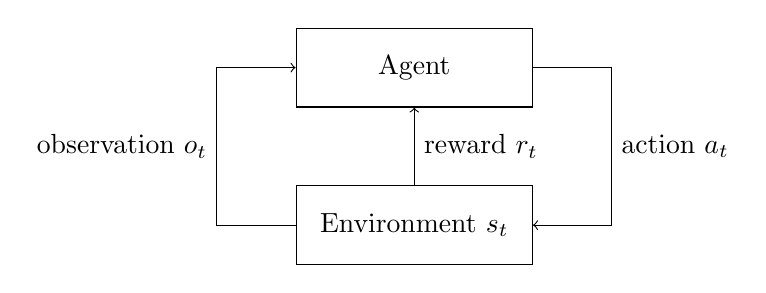
\begin{tikzpicture}[node distance=2cm]
    \tikzstyle{block} = [rectangle,minimum width=3cm,minimum height=1cm,text centered,draw=black,fill=white]
    \node (agent)[block]{Agent};
    \node (environment)[block,below of=agent]{Environment \(s_t\)};
    \draw [->] (agent.east) -- ++(1cm,0) -- node [anchor=west]{action \(a_t\)} ++(0,-2cm) -- (environment.east);
    \draw [->] (environment.north) -- node [anchor=west]{reward \(r_t\)} (agent.south);
    \draw [->] (environment.west) -- ++(-1cm,0) -- node [anchor=east]{observation \(o_t\)} ++(0,+2cm) -- (agent.west);
\end{tikzpicture}}
    \end{figure}
\end{frame}

\begin{frame}
    \frametitle{Reinforcement Learning II}

    \begin{itemize}
        \item Policy \(\pi(a|s)\) defines agent's behavior.
        % is a mapping from states to action probabilities.
        \item Find policy that maximizes expected future reward \(\mathbb{E} \left\lbrack \sum_{k=0}^{T} \gamma^{k-t-1} r_k \right\rbrack\).
        % Sum from the current time step.
        % Gamma is a discount factor.
        \item There are several different algorithms.
        % Each with their own advantages and disadvantages
        \item Reward signal is often a design parameter.
        % video games have inherent reward
        % in real world, no inherent reward
        % we have to design the reward so that the agent behaves desirably when the reward is maximized
        \item Deep reinforcement learning: approximate \(\pi\) with deep neural networks.
    \end{itemize}

    % The agent acts according to a policy that is a mapping from states to action probabilities.
    % Reinforcement learning is concerned with finding a policy that maximized the expected future reward.
    % In some cases there is some inherent reward signal (the goal is just to maximize the reward signal).
    % E.g. score in video games or goals in soccer.
    % Often, there is no reward signal. Instead, the reward signal is a design parameter that should tell the agent what its goal is.
    % Finally, deep reinforcement learning is an umbrella term for approaches in which the policy is approximated with deep neural networks.
\end{frame}

\subsection{Related Work}

\begin{frame}
    \frametitle{Related Work}

    \begin{itemize}
        \item Visual attention:
        % Determining what to pay attention to in an image
        \begin{itemize}
            \item Sequential focus points for foveated vision~\cite{mnih_recurrent_2014}.
        \end{itemize}
        \item Visual navigation:
        % Searching for some goal position in an environment
        \begin{itemize}
            \item Solve random mazes~\cite{mirowski_learning_2017}.
            \item Find target object in indoor scenes~\cite{zhu_target-driven_2017}.
        \end{itemize}
        \item Object detection:
        % Searching for objects in images
        \begin{itemize}
            \item Region proposals for object localization~\cite{caicedo_active_2015}.
            \item Anatomical landmark detection in medical images~\cite{ghesu_multi-scale_2019}.
        \end{itemize}
    \end{itemize}
    % Missing: how visual cues can guide search, overfitting and generalization from limited samples, rigorous performance evaluation.
\end{frame}